\documentclass[LaTeX2e,10pt,aspectratio=169]{beamer}
\setbeamertemplate{navigation symbols}{}
\usefonttheme[onlymath]{serif}

\usepackage{tikz}
\newcommand\w{0.12}

\usetikzlibrary{fit,positioning}
\tikzstyle{every picture}+=[remember picture]

\begin{document}

\bgroup
\setbeamercolor{background canvas}{bg=white}
\begin{frame}[plain]{}
	\begin{tikzpicture}[
    node distance = 7mm and -3mm,
every node/.style = {draw=black, rounded corners, fill=gray!30, 
                     minimum width=2cm, minimum height=0.5cm,
                     align=center}
                        ]
\node [label=Scarce Sinogram](scarceSinogram) {\includegraphics[width=\w\textwidth]{sophia_sin_example.png}};

\node (concat0)[right=5mm of scarceSinogram.east]{concatenation}; 

\node (generator)[right=5mm of concat0.east]{Generator}; 

\node [label=Inpainted Sinogram](inpainted)  [right=5mm of generator.east] {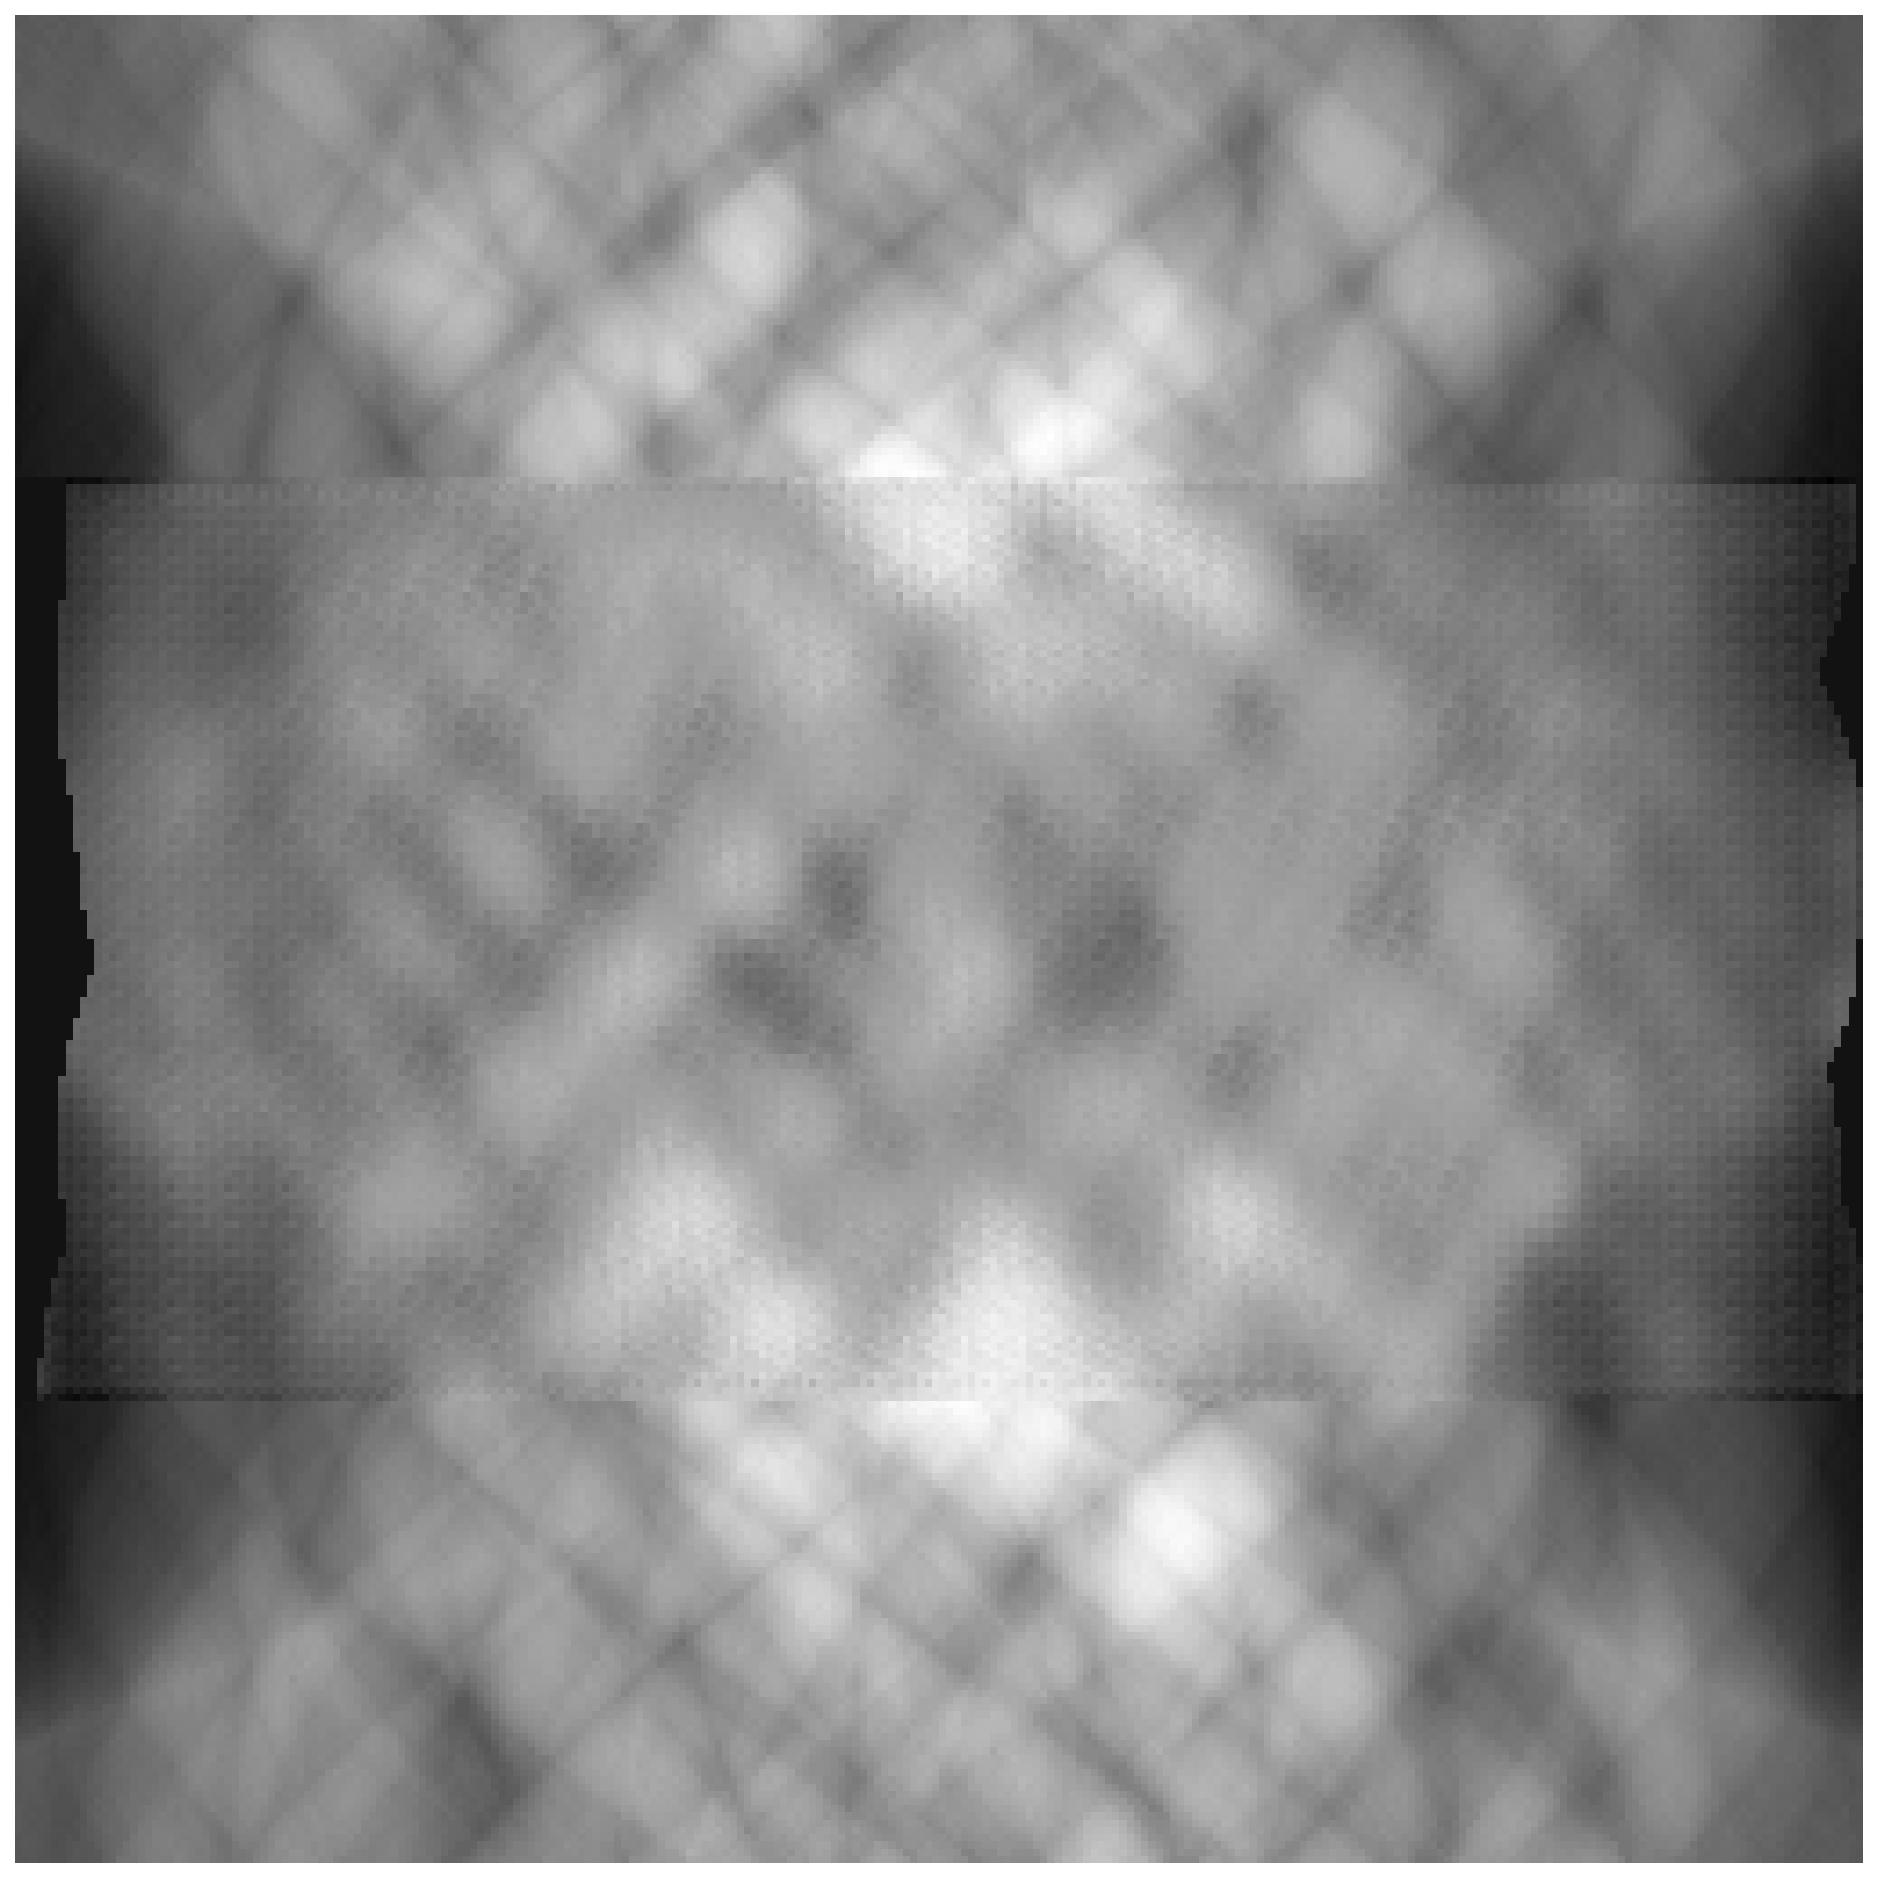
\includegraphics[width=\w\textwidth]{sinograms128_inferenceCadGan.jpg}};

\node [label={[shift={(0,-2.5)}]CAD Sinogram}](cadSinogram) [below=7.5mm of concat0.south] {\includegraphics[width=\w\textwidth]{cad_sin.png}};

\node [label={[shift={(0,-2.5)}]True Sinogram}](trueSinogram) [below right=5mm and 15mm of cadSinogram.south] {\includegraphics[width=\w\textwidth]{obj_sin.png}};

\node (concat1)[below=7.5mm of inpainted.south]{concatenation}; 

\node (concat2)[right=5mm of trueSinogram.east]{concatenation}; 

\node (detector)[minimum width=0.7cm, 
    minimum height=3cm, below right=17.5mm and 7mm of inpainted.east] {\rotatebox{90}{Detector}};
    
\node (false)[right=5mm of detector.65]{False}; 

\node (true)[right=5mm of detector.-65]{True};

\draw [-latex](scarceSinogram) -- (concat0);
\draw [-latex](cadSinogram) -- (concat0);
\draw [-latex](concat0) -- (generator);
\draw [-latex](generator) -- (inpainted);
\draw [-latex](inpainted) -- (concat1);
\draw [-latex](cadSinogram) -- (concat1);
\draw [-latex](cadSinogram.east) -- (concat2.north);
\draw [-latex](trueSinogram) -- (concat2);

\draw [-latex](concat1.east) -- (detector.115);
\draw [-latex](concat2.east) -- (detector.-115);

\draw [-latex](detector.65) -- (false);
\draw [-latex](detector.-65) -- (true);


\end{tikzpicture}
\end{frame}
\egroup


\end{document}